\documentclass[tikz,border=6pt]{standalone}
\usepackage{amsmath}
\usetikzlibrary{shapes.geometric,arrows.meta,positioning,fit,backgrounds}

\begin{document}
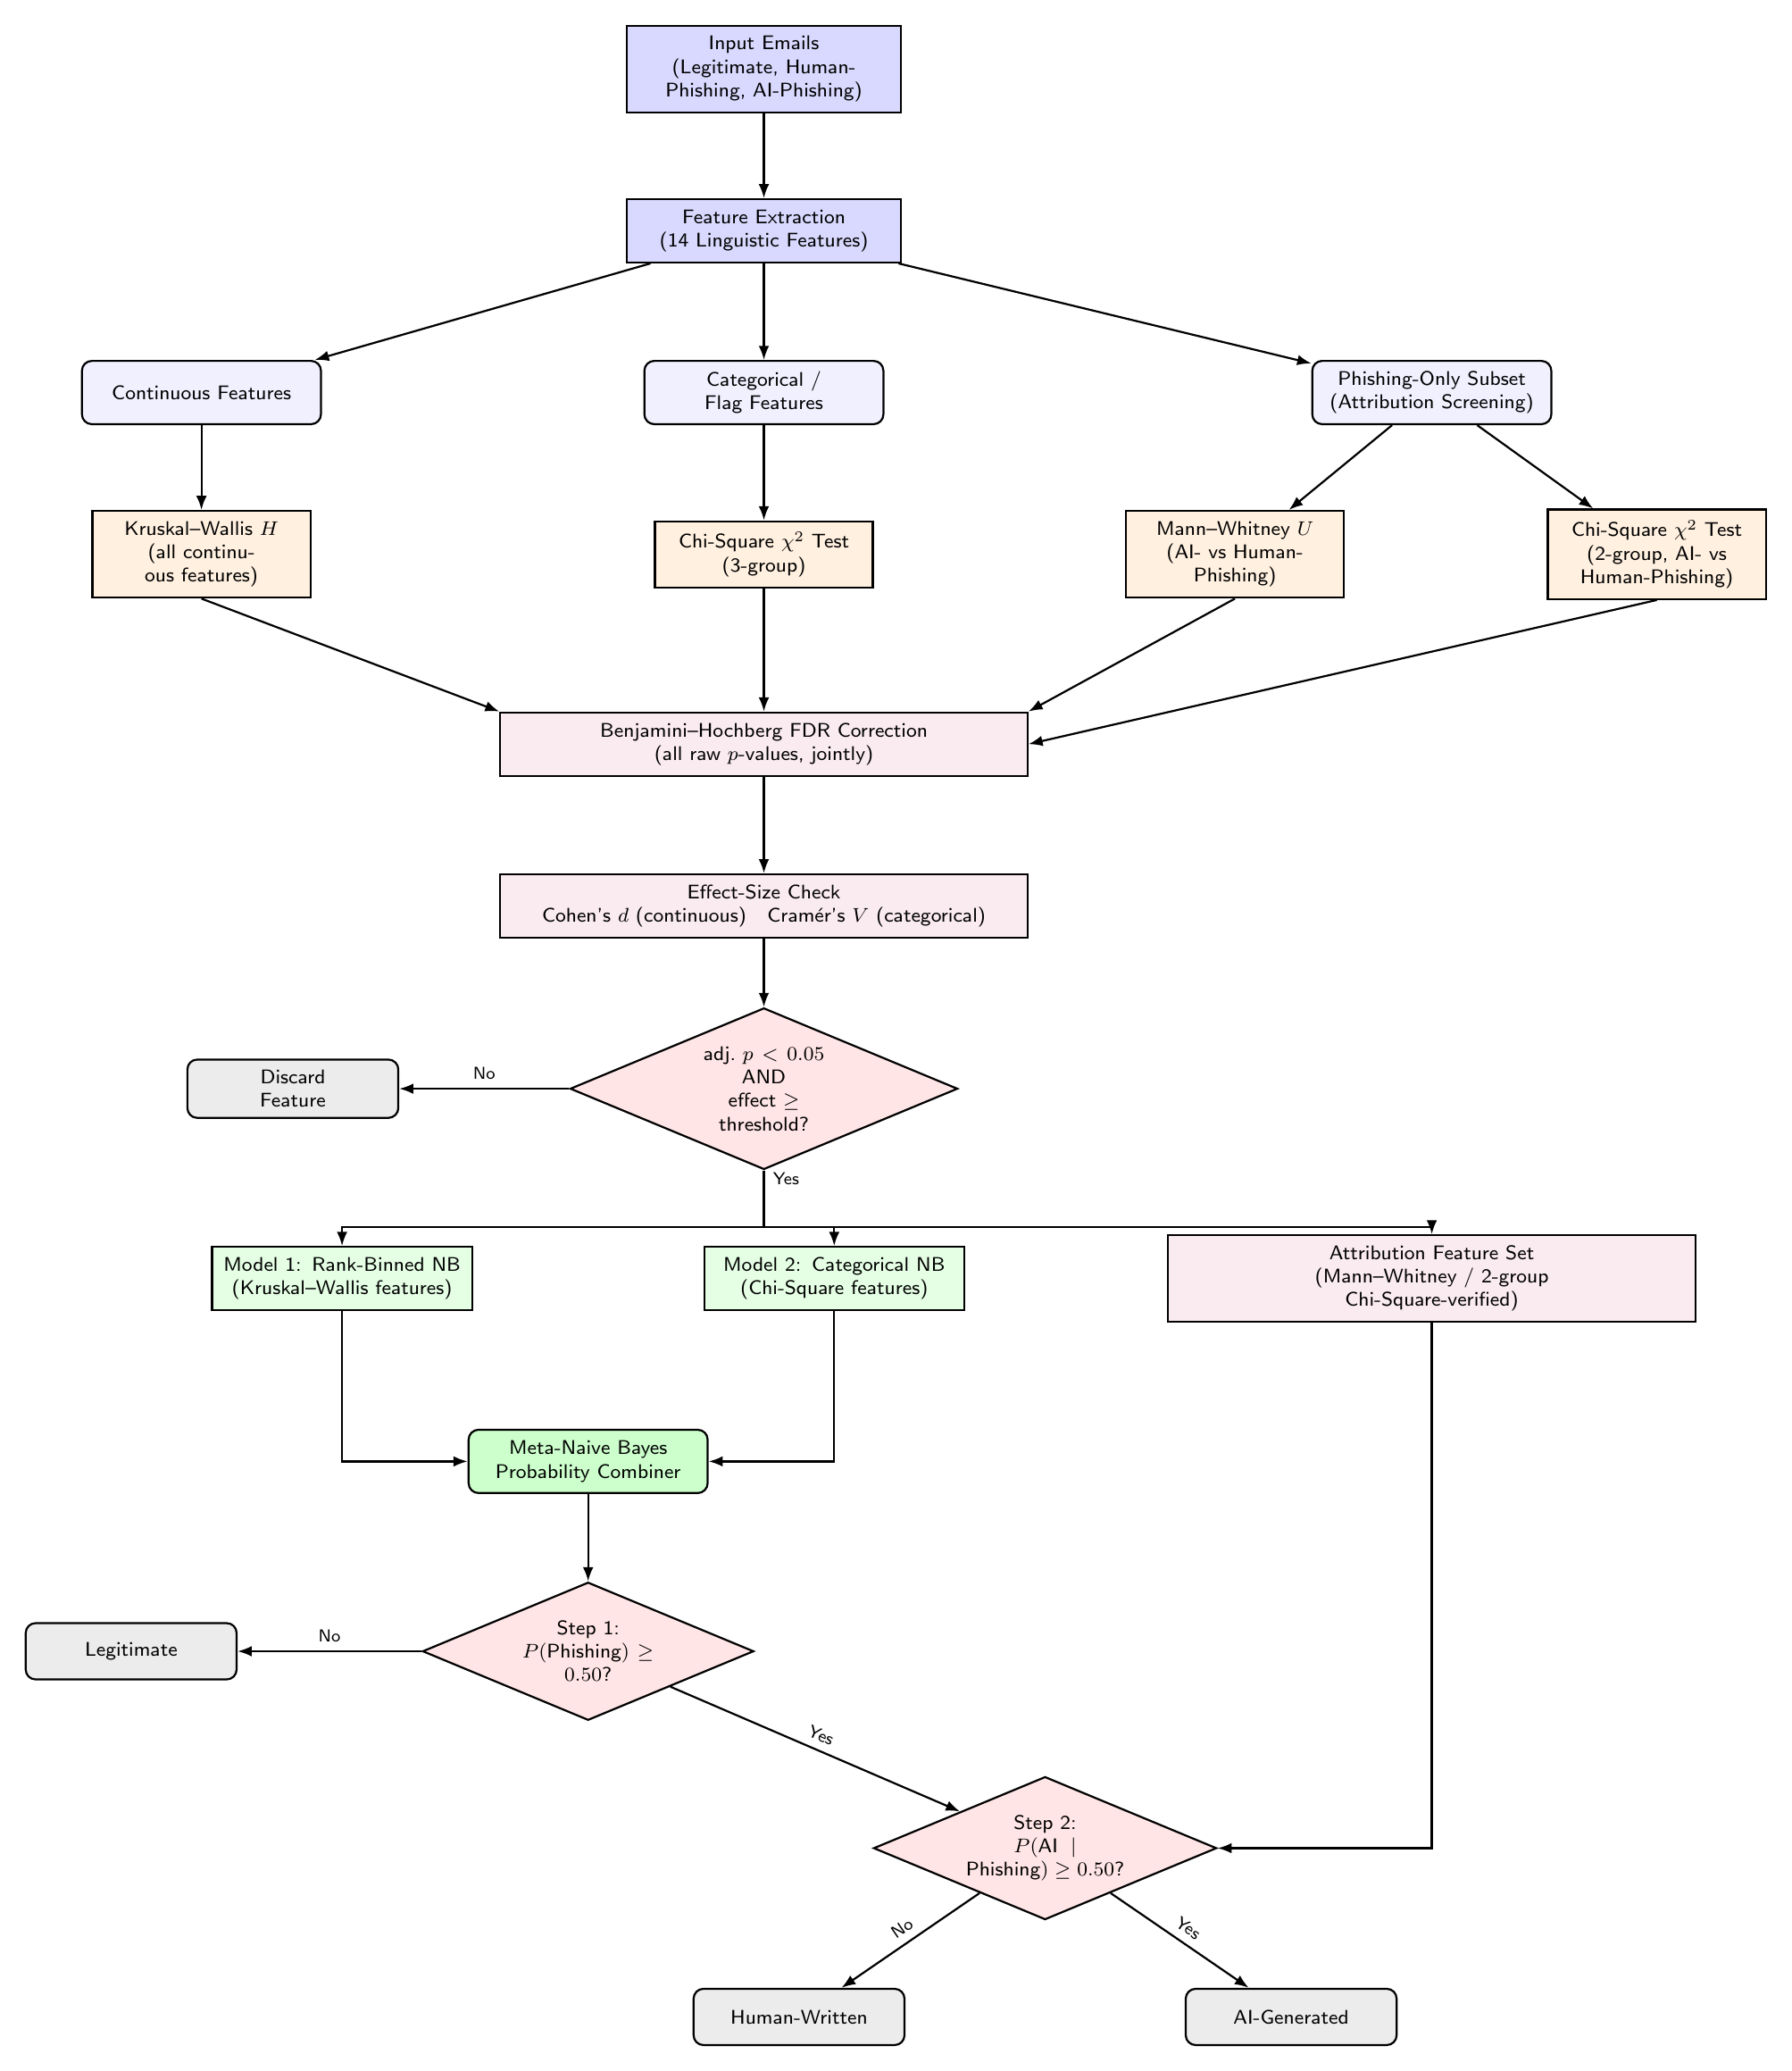
\begin{tikzpicture}[
    font=\sffamily\footnotesize,
    box/.style={rectangle, draw, thick, rounded corners, fill=blue!6,
                minimum height=0.9cm, text width=3.1cm, align=center, inner sep=1.5mm},
    io/.style={rectangle, draw, thick, fill=blue!15,
               minimum height=0.9cm, text width=3.6cm, align=center, inner sep=1.5mm},
    test/.style={rectangle, draw, thick, fill=orange!12,
                 minimum height=0.9cm, text width=2.8cm, align=center, inner sep=1.5mm},
    gate/.style={diamond, draw, thick, fill=red!10, aspect=2.4,
                 text width=2.3cm, align=center, inner sep=0.5mm},
    model/.style={rectangle, draw, thick, fill=green!10,
                  minimum height=0.9cm, text width=3.4cm, align=center, inner sep=1.5mm},
    term/.style={rectangle, draw, thick, rounded corners, fill=gray!15,
                 minimum height=0.8cm, text width=2.7cm, align=center, inner sep=1.5mm},
    conv/.style={rectangle, draw, thick, fill=purple!8,
                 minimum height=0.9cm, text width=7.2cm, align=center, inner sep=1.5mm},
    lbl/.style={font=\sffamily\scriptsize},
    arr/.style={-{Latex[length=2mm]}, thick},
]

% ===================== ROW 0-1: input / extraction =====================
\node[io] (input) at (0,0) {Input Emails\\(Legitimate, Human-Phishing, AI-Phishing)};
\node[io] (extract) at (0,-2.3) {Feature Extraction\\(14 Linguistic Features)};
\draw[arr] (input) -- (extract);

% ===================== ROW 2: three lanes =====================
\node[box] (contlane) at (-8,-4.6)   {Continuous Features};
\node[box] (catlane)  at (0,-4.6)    {Categorical / Flag Features};
\node[box] (attrlane) at (9.5,-4.6)  {Phishing-Only Subset\\(Attribution Screening)};
\draw[arr] (extract) -- (contlane);
\draw[arr] (extract) -- (catlane);
\draw[arr] (extract) -- (attrlane);

% ===================== ROW 3: tests (no normality branch — non-parametric only) ====
\node[test] (kw)     at (-8,-6.9)   {Kruskal--Wallis $H$\\(all continuous features)};
\node[test] (chisq3) at (0,-6.9)    {Chi-Square $\chi^2$ Test\\(3-group)};
\node[test] (mwu)    at (6.7,-6.9)  {Mann--Whitney $U$\\(AI- vs Human-Phishing)};
\node[test] (chisq2) at (12.7,-6.9) {Chi-Square $\chi^2$ Test\\(2-group, AI- vs\\ Human-Phishing)};

\draw[arr] (contlane) -- (kw);
\draw[arr] (catlane) -- (chisq3);
\draw[arr] (attrlane) -- (mwu);
\draw[arr] (attrlane) -- (chisq2);

% ===================== ROW 4: FDR convergence =====================
\node[conv] (fdr) at (0,-9.6) {Benjamini--Hochberg FDR Correction\\(all raw $p$-values, jointly)};
\draw[arr] (kw.south) -- (fdr.north west);
\draw[arr] (chisq3.south) -- (fdr.north);
\draw[arr] (mwu.south) -- (fdr.north east);
\draw[arr] (chisq2.south) -- (fdr.east);

% ===================== ROW 5: effect size =====================
\node[conv] (effsize) at (0,-11.9) {Effect-Size Check\\Cohen's $d$ (continuous)\quad Cram\'er's $V$ (categorical)};
\draw[arr] (fdr) -- (effsize);

% ===================== ROW 6: statistical gate =====================
\node[gate] (gateQ) at (0,-14.5) {adj.\ $p<0.05$\\AND\\effect $\geq$ threshold?};
\draw[arr] (effsize) -- (gateQ);

\node[term] (discard) at (-6.7,-14.5) {Discard\\Feature};
\draw[arr] (gateQ) -- node[lbl,above]{No} (discard);

% ===================== ROW 7: verified feature routing =====================
\node[model] (rbnb)   at (-6,-17.2)  {Model 1: Rank-Binned NB\\(Kruskal--Wallis features)};
\node[model] (cnb)    at (1,-17.2)   {Model 2: Categorical NB\\(Chi-Square features)};
\node[conv]  (attrset) at (9.5,-17.2) {Attribution Feature Set\\(Mann--Whitney / 2-group\\ Chi-Square-verified)};

\draw[arr] (gateQ.south) -- node[lbl,right,pos=0.15]{Yes} ++(0,-0.8) -| (rbnb.north);
\draw[arr] (gateQ.south) -- ++(0,-0.8) -| (cnb.north);
\draw[arr] (gateQ.south) -- ++(0,-0.8) -| (attrset.north);

% ===================== ROW 8: Meta-NB =====================
\node[box, fill=green!20] (meta) at (-2.5,-19.8) {Meta-Naive Bayes\\Probability Combiner};
\draw[arr] (rbnb.south) |- (meta.west);
\draw[arr] (cnb.south) |- (meta.east);

% ===================== ROW 9: Step 1 decision =====================
\node[gate] (step1) at (-2.5,-22.5) {Step 1:\\$P(\text{Phishing}) \geq 0.50$?};
\draw[arr] (meta) -- (step1);

\node[term] (legit) at (-9,-22.5) {Legitimate};
\draw[arr] (step1) -- node[lbl,above]{No} (legit);

% ===================== ROW 10: Step 2 decision =====================
\node[gate] (step2) at (4,-25.3) {Step 2:\\$P(\text{AI}\mid\text{Phishing}) \geq 0.50$?};
\draw[arr] (step1) -- node[lbl,above,sloped]{Yes} (step2);
\draw[arr] (attrset.south) |- (step2.east);

\node[term] (human) at (0.5,-27.7) {Human-Written};
\node[term] (ai)    at (7.5,-27.7) {AI-Generated};
\draw[arr] (step2) -- node[lbl,above,sloped]{No} (human);
\draw[arr] (step2) -- node[lbl,above,sloped]{Yes} (ai);

\end{tikzpicture}
\end{document}
